\chapter{Error Representations and Three-dimensional Rigid Transformation}
\label{chap:Error Representations and Three-dimensional Rigid Transformation}

In this section some basic knowledge of mathematics, which are related to this thesis, would be introduced.

\section{Error representations}

\subsection{Norms}
%TODO 
\textbf{Vector Norm:}

A vector norm is a measure for the size of a vector, on a real or complex vector space V is a mapping $V \to \mathbb{R} $ with following properties:

\begin{enumerate}
\item $ \norm{v} \geq 0 \quad \forall v $
\item $ \norm{v} = 0 \quad \Leftrightarrow  \quad v = 0$
\item $ \norm{\alpha v} = |\alpha| \norm{v} $
\item $ \norm{v+w} \leq  \norm{v} + \norm{w}$
\end{enumerate}

\textit{1-norm}:\\
The sum of the absolute values of all elements of vector \textit{v}.
\begin{equation*}  
\norm{v}_1 = \sum_{i=1}^{n} |v_{i}|   
\end{equation*}

\textit{2-norm}:\\
The square root of the sum of all absolute values from vector \textit{v}.
\begin{equation*}  
\norm{v}_2 = (\sum_{i=1}^{n} |x_{i}|^2)^{\frac{1}{2}}     
\end{equation*}

\textit{$\infty$-norm}:\\
The maximum value of all elements of vector \textit{v}.
\begin{equation*}  
\norm{v}_{\infty} =
 \operatorname*{max}_i |v_i|    
\end{equation*}

\textit{p-norm}:\\
The the 1/p power of the sum of p-th power of all vector elements.
\begin{equation*}  
\norm{v}_p =
 (\sum_{i=1}^{n} |v_i|^p)^{\frac{1}{p}}   
\end{equation*}



\textbf{Matrix Norm:}\\
A matrix norm has following properties:

\begin{enumerate}
\item $ \norm{A} \geq 0 \quad \forall A $
\item $ \norm{A} = 0 \quad \Leftrightarrow  \quad A = 0$
\item $ \norm{\alpha A} = |\alpha| \norm{A} $
\item $ \norm{A+B} \leq  \norm{A} + \norm{B}$
\item $ \norm{A \cdot B} \leq  \norm{A} \cdot \norm{B}$
\end{enumerate}
 
First, assume that we have a $m \times n$ matrix \textit{A}(m rows, n columns).

\textit{1-norm}:\\
The maximum value of the sum of the absolute values from column vectors of matrix.
\begin{equation*}  
\norm{A}_1 =
 \operatorname*{max}_j \sum_{i=1}^{m} |a_{ij}|   
\end{equation*}

\textit{2-norm}:\\
The square root of the maximum eigenvalue of matrix $A^TA$ .
\begin{equation*}  
\norm{A}_2 = \sqrt{\lambda_1}
\end{equation*}

\textit{$\infty$-norm}:\\
The maximum value of the sum of the absolute values from row vectors of matrix.
\begin{equation*}  
\norm{A}_{\infty} =
 \operatorname*{max}_j \sum_{i=1}^{n} |a_{ij}|   
\end{equation*}

\textit{F-norm(Frobenius-norm)}:\\
F-norm is also call Euclidean norm, is the square root of the sum of the absolute squares of matrix elements.
\begin{equation*}  
\norm{A}_F =
 (\sum_{i=1}^{m} \sum_{j=1}^{n} |a_{ij}|^2)^{\frac{1}{2}}   
\end{equation*}


\subsection{SVD}

Any matrix $m \times n$ $A$ can be factored as 
\begin{equation*}  
A = U \Sigma V^*,  
\end{equation*}
where \textbf{U}($m \times m$), \textbf{V}($n \times n$) are unitary matrix and $\mathbf{\Sigma}$ is a diagonal $m \times n$ with non-negative real number, $\mathbf{V^*}$ is the conjugate transpose of $\mathbf{V}$.

The \textbf{singular values} of \textbf{A} are the square root of the eigenvalues of $A^*A$:
\begin{equation*}  
  \sigma_1 \geq \sigma_2 \geq \dotso \geq \sigma_m \geq 0
\end{equation*}
The eigenvectors of $A^*A$ consist of the columns of \textbf{V}. The eigenvectors of $AA^*$ consist of the columns of \textbf{U}.


\subsection{Condition number}
In the field of numerical analysis, the condition number of a function with respect to an argument measures how much the output value of the function can change for a small change in the input argument. This is used to measure how sensitive a function is to changes or errors in the input, and how much error in the output results from an error in the input\cite{wiki_cn}. 
% https://en.wikipedia.org/wiki/Condition_number

We now consider a system of linear equation $Ax = b$.
\begin{align*}  
Ax &= b \\
A(x + \Delta x) &= (b + \Delta b)
\end{align*}

The condition number is:
\begin{align*}  
\kappa = \operatorname*{max}_{\Delta b}\frac{\norm{\Delta x}/\norm{x}}{\norm{\Delta b}/\norm{b}}
\end{align*}

We find that
\begin{align*}  
\kappa \leq \norm{A} \cdot \norm{A^{-1}}
\end{align*}
And we can find a specific $\Delta b$ to satisfy this bound:
\begin{align*}  
\kappa = \norm{A} \cdot \norm{A^{-1}}
\end{align*}
For the 2-norm, the condition number is the ratio of maximal and minimal singular values of $A$ respectively.
\begin{align*}  
\kappa = \frac{\sigma_{max}{(A)}}{\sigma_{min}{(A)}},
\end{align*}

\subsection{Root mean square error}
\textbf{Root mean square error}(\textbf{RMSE}) error is a useful representation of errors in measurement systems. The \textbf{RMSE} is used to measure the sample standard deviation of the differences between predicted and observed values. In this thesis \textbf{RMSE} is a measure of accuracy.
\begin{align*}  
e_{rms} = \sqrt{\frac{1}{N}\sum_{i=1}^{N}|x-x_i|^2}
\end{align*}

\section{Three-dimensional rigid transformation}
The space in our daily life is three-dimensional and we are naturally accustomed to the movement of three-dimensional space. Three-dimensional space consists of three axes, so the position of one point in 3D can be described with 3 axes. However, the rigid body we are considering now, it not only has a position but also has his own pose. The camera can also be seen as a rigid body in 3D, so the \textit{position} refers to where the camera is in space, and the \textit{pose} refers to the orientation of the camera.

In mathematics, we use rigid transformation to describe the motion of a rigid object in n-dimensional space. In general, the rigid transformations include rotations, translations, reflections, or their combination. To avoid ambiguity, in this thesis the rigid transformation can be only decomposed as a rotation followed by a translation. Any object will keep the same shape and size after a rigid transformation\cite{wiki_rt}.
% https://en.wikipedia.org/wiki/Rigid_transformation
 
\subsection{Euclidean transformation between coordinate systems}

Recall that a vector in 3D can be represented with 3 numbers in $R^3$. If we determine a coordinate system, which means we can get three linearly independent basis vectors $(e1, e2, e3)$, then we can represent the vector as a linear combination of $(e1, e2, e3)$:

\begin{equation*}
 v = 
     \begin{bmatrix} e_1 & e_2 & e_3 \end{bmatrix} 
     \begin{bmatrix} a_1 \\ a_2 \\ a_3 \end{bmatrix}
   = a_1e_1 + a_2e_2 + a_3e_3               
\end{equation*}

We can use outer product to represent the rotation of a vector. For example: $w = a \times b$. The rotation from a to b can be described with w.
Similar to the rotation of vectors, we can also represent the relationship of rotation between two coordinate systems and adding translation, they are seen to be as the transformation relationship between coordinate systems. During the robot's movement, the usual method is to set an inertial coordinate system(or called world coordinate system), we can assume that the world coordinate system is fixed, as shown in figure \ref{fig:wcT} $X_W, Y_W, Z_W$. At the same time, the camera or robot is a moving coordinate system, as shown in figure \ref{fig:wcT} $X_C, Y_C, Z_C$. The movement of camera is a rigid body movement, it guarantees that the length and angle of the same vector will not change in each coordinate system(euclidean transformation). For one vector \textit{p}, the coordinates of \textit{p} in world coordinate system and in camera coordinate system are not same, the transformation can be described with transform matrix T.

\begin{figure}[h]
\centering
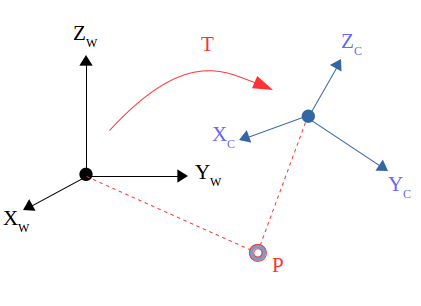
\includegraphics[scale=0.5]{./fig/wcT.png}
\caption{Transformation between coordinate systems}
\label{fig:wcT}
\end{figure}

One euclidean transformation consists of rotation and translation. First we consider rotation, we assume that one orthonormal basis $(e_1, e_2, e_3)$ after rotating becomes $(e_1^{\prime}, e_2^{\prime}, e_3^{\prime})$. In this way, for one same vector \textit{a}(this vector does not move!), the coordinates of vector \textit{a} in both system are $\begin{bmatrix} a_1,& a_2,& a_3 \end{bmatrix}^T$ and $\begin{bmatrix} a_1^{\prime}, & a_2^{\prime}, & a_3^{\prime} \end{bmatrix}^T$. According to the definition of coordinate we get:

\begin{equation*}\label{equet1}
 \begin{bmatrix} e_1 & e_2 & e_3 \end{bmatrix} 
 \begin{bmatrix} a_1 \\ a_2 \\ a_3 \end{bmatrix}
 = 
     \begin{bmatrix} e_1^{\prime} & e_2^{\prime} & e_3^{\prime} \end{bmatrix} 
     \begin{bmatrix} a_1^{\prime} \\ a_2^{\prime} \\ a_3^{\prime} \end{bmatrix}             
\end{equation*}

In order to describe the relationship of both coordinate systems, the above equation should multiply by $\begin{bmatrix} e_1^T \\ e_2^T \\ e_3^T \end{bmatrix}$ on both left and right sides, and we get a unit matrix on the left side:

\begin{equation}\label{eq:equet2}
 \begin{bmatrix} a_1 \\ a_2 \\ a_3 \end{bmatrix}
 = 
     \begin{bmatrix} e_1^Te_1^{\prime} & e_1^Te_2^{\prime} & e_1^Te_3^{\prime}\\
                     e_2^Te_1^{\prime} & e_2^Te_2^{\prime} & e_2^Te_3^{\prime}\\
                     e_3^Te_1^{\prime} & e_3^Te_2^{\prime} & e_3^Te_3^{\prime}
     \end{bmatrix}      
     \begin{bmatrix} a_1^{\prime} \\ a_2^{\prime} \\ a_3^{\prime} \end{bmatrix}             
 = Ra^{\prime}    
\end{equation}

So the matrix \textit{R} from equation \ref{eq:equet2} is called \textbf{rotation matrix}. We can find that the rotation matrix is composed of the inner product of two sets of orthonormal bases, it represents the transformation relationship of one same vector before and after rotating. we can use rotation matrix to describe camera rotation.

In addition to rotation there is also translation in euclidean transformation. One vector \textit{a} in world coordinate system becomes \textit{$a^{\prime}$} after one time rotation and one time translation \textit{t}, we can combine both rotation and translation as:

\begin{equation*}
a^{\prime} = Ra + t
\end{equation*}

Through the above formula, we describe coordinate transformation with rotation matrix \textit{R} and translation vector \textit{t} in euclidean space completely. 


\subsection{Elemental rotation matrix}
A elemental rotation is a rotation about one of the axes of a coordinate system. The following elemental rotation matrix rotates vectors by an angle $\alpha$ about the x-axis in three dimensions and the right-hand rule is used.

\texttt{Right-hand rule}: right thumb points along the axis of rotation in the positive direction, and the direction of the rest curved fingers corresponds to the positive rotation direction.

\begin{figure}[h]
\centering
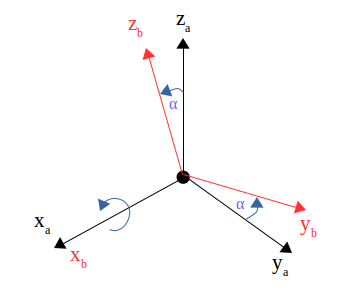
\includegraphics[scale=0.5]{./fig/rotationx.png}
\caption{Rotation about x-axis by angle $\alpha$}
\label{fig:rotationx}
\end{figure}

\begin{equation*}
R_x(\alpha) = R(x;\alpha)
      = \begin{bmatrix} 1 & 0 & 0\\
                        0 & cos(\alpha) & -sin(\alpha)\\
                        0 & sin(\alpha) & cos(\alpha) \end{bmatrix}                
\end{equation*}

Analog formulas also work for the elemental rotation matrix by an angle $\beta$, $\gamma$ about the \textit{y}-axis and \textit{z}-axis in 3D.
\begin{equation*}
R_y(\beta) = R(y;\beta)
      = \begin{bmatrix} cos(\beta) & 0 & sin(\beta)\\
                        0 & 1 & 0\\
                        -sin(\beta) & 0 & cos(\beta) \end{bmatrix}                
\end{equation*}
 
\begin{equation*}
R_z(\gamma) = R(z;\gamma)
      = \begin{bmatrix} cos(\gamma) & -sin(\gamma) & 0\\
                        sin(\gamma) & cos(\gamma) & 0\\
                        0 & 0 & 1 \end{bmatrix}                
\end{equation*}

\subsection{Euler angles}
The Euler angles are three angles to describe the orientation of a rigid body with respect to a fixed coordinate system. They can also represent the orientation of a mobile frame of reference in physics or the orientation of a general basis in 3-dimensional linear algebra. Any orientation can be achieved by composing three elemental rotations, i.e. rotations about the axes of a coordinate system. Euler angles can be defined by three of these rotations\cite{wiki_ea}.
% WIKI https://en.wikipedia.org/wiki/Euler_angles

In this thesis we denote euler angles as $\alpha$, $\beta$, $\gamma$

The three elemental rotations may be extrinsic (rotations about the axes xyz of the original coordinate system, which is assumed to remain motionless), or intrinsic (rotations about the axes of the rotating coordinate system XYZ, solidary with the moving body, which changes its orientation after each elemental rotation)\cite{wiki_ea}.
% WIKI https://en.wikipedia.org/wiki/Euler_angles

In general, euler angels can be divided in two groups(Proper Euler angles and Tait-Bryan angles):

\begin{itemize}
\item Proper Euler angles:

\begin{center}
    \begin{tabular}{ | l | l | l | p{5cm} |}
    \hline
      & Intrinsic rotations & Extrinsic rotations\\ \hline 
    1 & $z-x^{\prime}-z^{\prime\prime}$ & $z-x-z$ \\ \hline
    2 & $x-y^{\prime}-x^{\prime\prime}$ & $x-y-x$ \\ \hline
    3 & $y-z^{\prime}-y^{\prime\prime}$ & $y-z-y$ \\ \hline
    4 & $z-y^{\prime}-z^{\prime\prime}$ & $z-y-z$ \\ \hline
    5 & $x-z^{\prime}-x^{\prime\prime}$ & $x-z-x$ \\ \hline
    6 & $y-x^{\prime}-y^{\prime\prime}$ & $y-x-y$ \\ \hline
    \end{tabular}
\end{center}

\item Tait-Bryan angles(Tait-Bryan angles are also called yaw, pitch, and roll)

\begin{center}
    \begin{tabular}{ | l | l | l | p{5cm} |}
    \hline
      & Intrinsic rotations & Extrinsic rotations\\ \hline 
    1 & $x-y^{\prime}-z^{\prime\prime}$ & $x-y-z$ \\ \hline
    2 & $y-z^{\prime}-x^{\prime\prime}$ & $y-z-x$ \\ \hline
    3 & $z-x^{\prime}-y^{\prime\prime}$ & $z-x-y$ \\ \hline
    4 & $x-z^{\prime}-y^{\prime\prime}$ & $x-z-y$ \\ \hline
    5 & $z-y^{\prime}-x^{\prime\prime}$ & $z-y-x$ \\ \hline
    6 & $y-x^{\prime}-z^{\prime\prime}$ & $y-x-z$ \\ \hline
    \end{tabular}
\end{center}
\end{itemize}

\begin{equation*}
 \text{Proper Euler angles} 
 \left\{
 \begin{aligned}
        \text{Intrinsic rotations: $\overbrace{R = Z_1(\alpha)X_2(\beta)Z_3(\gamma)}^\text{post-multiply: $Z_1 \to X_2' \to Z_3''$}$}\\
        \text{Extrinsic rotations: $\underbrace{R = Z_3(\alpha)X_2(\beta)Z_1(\gamma)}_\text{pre-multiply: $Z_1 \to X_2 \to Z_3$}$}
 \end{aligned}
 \right.\
 \qquad
\end{equation*}

\begin{equation*}
 \text{Tait Bryan angles} 
 \left\{
 \begin{aligned}
        \text{Intrinsic rotations: $\overbrace{R = X_1(\alpha)Y_2(\beta)Z_3(\gamma)}^\text{post-multiply: $X_1 \to Y_2' \to Z_3''$}$}\\
        \text{Extrinsic rotations: $\underbrace{R = X_3(\alpha)Y_2(\beta)Z_1(\gamma)}_\text{pre-multiply: $Z_1 \to Y_2 \to X_3$}$}
 \end{aligned}
 \right.\
 \qquad
\end{equation*}

There are two interpretations for chained rotations:
\begin{itemize}
\item pre-multiply: $R = (R_n \cdot (R_{n-1} \cdot ... \cdot (R_2 \cdot R_1))))$, rotation in the order 1, 2, ...,n-1, n
\item post-multiply: $R = (((R_n \cdot R_{n-1}) \cdot ...R_2) \cdot R_1)$, rotation in the order n, n-1, ..., 2, 1
\end{itemize}

Sometimes, all kinds of sequences from \textit{Proper Euler angles} and \textit{Tait-Bryan angles} are called "Euler angles". In this thesis we give a example of derivation for \textit{Proper Euler angles, intrinsic rotations}:

\begin{equation}
\begin{aligned}
R &= R(z;\alpha)R(y;\beta)R(z;\gamma)
  = \begin{bmatrix} R_{11} & R_{12} & R_{13}\\
                     R_{21} & R_{22} & R_{23}\\
                     R_{31} & R_{32} & R_{33} \end{bmatrix} \\                  
      &= \begin{bmatrix} cos(\alpha)cos(\beta)cos(\gamma)-sin(\alpha)sin(\gamma) & -cos(\alpha)cos(\beta)sin(\gamma)-sin(\alpha)cos(\gamma) & cos(\alpha)sin(\beta)\\
                         sin(\alpha)cos(\beta)cos(\gamma)+cos(\alpha)sin(\gamma) & -sin(\alpha)cos(\beta)sin(\gamma)+cos(\beta)cos(\gamma)  & sin(\alpha)sin(\beta) \\
                         -sin(\beta)cos(\gamma) & sin(\theta)sin(\gamma) & cos(\beta) \end{bmatrix}   
\end{aligned}                   
\end{equation}

\subsection{Transform matrix and homogeneous matrix representation}
In our case, we use rigid transformation to describe the 3D spacial transformation of one spacial point between two different coordinate systems, which is shown in figure \ref{fig:rt}.

\begin{figure}[h]
\centering
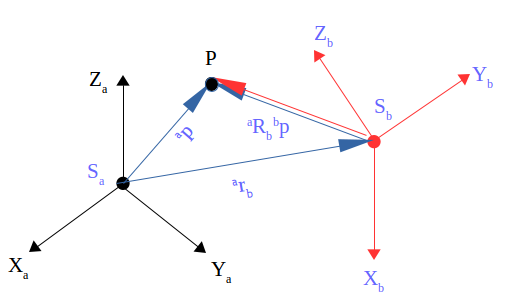
\includegraphics[scale=0.5]{./fig/rt.png}
\caption{Transformation from $S_a$ to $S_b$}
\label{fig:rt}
\end{figure}

And the transformation of point \textit{P} from $S_a$ to $S_b$ is:
\begin{align}\label{eq:equTM1}
\Aboxed{ \tensor*[^a]{p}{} = \tensor*[^a]{r}{_b} + \tensor*[^a]{R}{_b}\tensor*[^b]{p}{}}
\end{align}

\begin{itemize}
\item $\tensor*[^a]{p}{} \in \mathbb{R}^{3}$: P coordinate in system $S_a$
\item $\tensor*[^b]{p}{} \in \mathbb{R}^{3}$: P coordinate in system $S_b$
\item $\tensor*[^a]{r}{_b} \in \mathbb{R}^{3}$: translation-vector
\item $\tensor*[^a]{R}{_b} \in \mathbb{R}^{3\times3}$: rotation between $S_a$ and $S_b$
\end{itemize}

Equation \ref{eq:equTM1} represents the rotation and translation in euclidean space. But there is still a little problem: the transformation is not linear. We assume that we make two times rotations continuously: $R_1, t_1$ and $R_2, t_2$:

\begin{align*}\label{eq:equTM2}
     b = R_1a + t_1, c = R_2a + t_2               
\end{align*}

But the transformation from $a$ to $c$ is:

\begin{equation*}
     c = R_2(R_1a + t_1) + t_2            
\end{equation*}

This kind of form is too complicated after many times transformations. We turn the n-dimensional euclidean space from $R^n$ to $n+1$-dimensional by adding 1 at the end of the n-dimensional vector. It is called homogeneous coordinate.


\begin{equation*}
     \begin{bmatrix} x^{\prime} \\ 1 \end{bmatrix}
     =
     \begin{bmatrix} R & t\\
                     0^{T} & 1 \end{bmatrix}
     \begin{bmatrix} x \\ 1 \end{bmatrix}
     = T    
     \begin{bmatrix} x \\ 1 \end{bmatrix}                        
\end{equation*}

The matrix \textbf{T} is called \textbf{Transform Matrix}. Now we get a linear transformation which additionally fulfills the requirements of additivity and homogeneity, this matrix representation is easier to use. Through matrix product of the respective homogeneous matrices we can compute the concatenation of multiple rigid transformations. 

